\chapter{Computational efficiency}\label{ch:complexity}

\begin{remark}{Outline}
In this chapter, we study the computational efficiency of tree-based ensemble
methods. In sections~\ref{sec:5:complexity-fit} and \ref{sec:5:complexity-predict},
we derive and discuss the time complexity of random forests, first for building them from data and then for making predictions. In
Section~\ref{sec:5:impl}, we discuss technical details that are critical
for efficiently  implementing random forests. Finally, we conclude in
Section~\ref{sec:5:benchmarks} with benchmarks of the random forest implementation developed
within this work and compare our solution with alternative implementations.
\end{remark}

\section{Complexity of the induction procedure}
\label{sec:5:complexity-fit}

The dominant objective of most machine learning methods is to find models that
maximize accuracy. For models of equivalent performance, a secondary objective
is usually to minimize complexity. Complexity, however, has many facets. A
first and immediate notion of complexity in decision trees and random forests is
the \textit{time complexity} for learning models, that is the number of
operations required for building models from data.

Given the exponential growth in the number of possible partitions of $N$
samples, we chose in Section~\ref{sec:3:splitting-rules} to restrict splitting
rules to binary splits defined on single variables. Not only this is sufficient
for reaching good accuracy (as discussed in Section~\ref{sec:4:consistency}),
it also allows for time complexity to effectively remain within reasonable bounds.

Formally, let $T(N)$ denotes the time complexity for building a decision tree from a
learning set ${\cal L}$ of $N$ samples. From Algorithm~\ref{algo:induction},
$T(N)$ corresponds to the number of operations required for splitting a node of $N$ samples and then for recursively
building two sub-trees respectively from $N_{t_L}$ and $N_{t_R}$ samples. Without
loss of generality, let us assume that the learning samples all have distinct
input values, such that it is possible to build a fully developed decision tree
where each leaf contains exactly one sample. Under this assumption, determining
time complexity therefore amounts to solve the recurrence equation
\begin{equation}\label{eqn:complexity:rec}
\begin{cases}
T(1) = O(1) \\
T(N) = c(N) + T(N_{t_L}) + T(N_{t_R}),
\end{cases}
\end{equation}
where $c(N)$ is the time complexity for splitting a node of $N$ samples. For
$N=1$, the node is necessarily pure, hence the constant time complexity $O(1)$.
For $N>1$, $c(N)$ corresponds to the time complexity for finding a split $s$
and then partitioning the node samples into ${t_L}$ and ${t_R}$. This later
operation requires at least to iterate over all $N$ samples, which sets a
linear lower bound on time complexity within a node, i.e., $c(N)=\Omega(N)$. As
for finding the split $s$, this can be achieved in several ways, as outlined in
the previous chapters  for several randomized variants of the induction
procedure. As we will see, not only this is an impact on the accuracy of the
resulting model, it also drives the time complexity of the induction procedure.

\begin{remark}{Big O notations}
Time complexity analyzes the asymptotic behavior of an algorithm
with respect to the size $N$ of its input and its hyper-parameters. In this way,
big O notations are used to formally express an asymptotic upper bound on the
growth rate of the number $f(N)$ of steps in the algorithm. Formally,
we write that
\begin{equation}
f(N) =  O(g(N)) \ \text{if}\ \exists c > 0, N_0 > 0, \forall N > N_0, f(N) \leq c g(N)
\end{equation}
to express that  $f(N)$ is asymptotically upper bounded by $g(N)$, up to some neglectable constant factor $c$.
Similarly, big $\Omega$ notations are used to express an asymptotic lower
bound on the growth rate of the number of steps in the algorithm. Formally,
we write that
\begin{equation}
f(N) =  \Omega(g(N)) \ \text{if}\ \exists c > 0, N_0 > 0, \forall N > N_0,  c g(N) \leq f(N)
\end{equation}
to express that $f(N)$ is asymptotically lower bounded by $g(N)$.
Consequently, if $f(N)$ is both $O(g(N))$ and $\Omega(g(N))$ then $f(N)$ is
both lower bounded and upper bounded asymptotically by $g(N)$ (possibly for different constants),
which we write using big $\Theta$ notations:
\begin{equation}
f(N) = \Theta(g(N)) \ \text{if}\  f(N) =  O(g(N)) = \Omega(g(N)).
\end{equation}
\end{remark}

In the original CART induction procedure~\citep{breiman:1984}
(Algorithms~\ref{algo:findsplit} and \ref{algo:findsplit:x_j}), finding a split
$s$  requires, for each of the $p$ variables $X_j$ (for $j=1,\dots,p$), to sort
the values $x_{i,j}$ of all $N$ node samples (for $i=1,\dots,N$) and then to
iterate over these in order to find the best threshold $v$. The most costly
operation is sorting, whose time complexity is at worst $O(N \log N)$. As a
result, the overall within-node complexity is $c(N) = O(p N \log N)$. In a
randomized tree as built with the Random Forest algorithm~\citep{breiman:2001}
(RF, Algorithm~\ref{algo:findsplit:random}), the search of the best split $s$
is carried out in the same way, but only on $K \leq p$ of the input variables,
resulting in a within-node complexity $c(N) = O(K N \log N)$. In Extremely
Randomized Trees~\citep{geurts:2006} (ETs, Algorithm~\ref{algo:findsplit:et}),
discretization thresholds are drawn at random within the minimum and maximum
node sample values of $X_j$, making sort no longer necessary. As such, the
within-node complexity reduces to the time required for finding these lower and
upper bounds, which can be done in linear time, hence $c(N)=O(KN)$. Finally, in
Perfect Random Tree Ensembles~\citep{cutler:2001} (PERT,
Algorithm~\ref{algo:findsplit:pert}), cut-points $v$ are set midway between
two randomly drawn samples, which can be done in constant time, independently
of the number $N$ of node samples. Yet, the within-node complexity is lower
bounded by the time required for partitioning the node samples into ${t_L}$ and
${t_R}$, hence $c(N)=O(N)$.

Since both CART and PERT can respectively be considered as special cases of RF
and ETs with regards to time complexity (i.e., for $K=p$ in CART, for $K=1$ in
PERT), let us consider the overall complexity $T(n)$ when either
$c(N)=O(KN\log N)$ or $c(N)=O(KN)$ (for $K=1,\dots,p$). Time complexity
is studied in three cases:

\begin{description}
\item \textit{Best case.}\hfill\\
      The induction procedure is the most effective
      when node samples can always be partitioned into two balanced subsets of $\tfrac{N}{2}$
      samples.

\item \textit{Worst case.}\hfill\\
      By contrast, the induction procedure is the least
      effective when splits are unbalanced. In the worst case,
      this results in splits that move a single sample in the first sub-tree and
      all $N-1$ others in the second sub-tree.

\item \textit{Average case.}\hfill\\
      The average case corresponds to the average time
      complexity, as taken over all possible learning sets ${\cal L}$ and
      all random seeds $\theta$.  Since the analysis of this case is hardly
      feasible without strong assumptions on the structure of the problem,
      we consider instead the case where the sizes of the possible
      partitions of a node are all equiprobable.

\end{description}

\begin{remark}{Master Theorem}
Some of the results outlined in the remaining of this section make use of the
Master Theorem~\citep{goodrich:2006}, which recall below to be self-contained.

\begin{theorem}
Let consider the recurrence equation
\begin{equation}
\begin{cases}
T(1) = c & \text{if}\quad n < d\\
T(n) = aT(\frac{n}{b}) + f(n) & \text{if}\quad n \geq d
\end{cases}
\end{equation}
where $d \geq 1$ is an integer constant, $a > 0$, $c>0$ and $b>1$ are real constants, and
$f(n)$ is a function that is positive for $n \geq d$.

\begin{enumerate}
\item If there is a small constant $\epsilon > 0$, such that $f(n)$ is $O(n^{\log_b a - \epsilon})$, then $T(n)$ is $\Theta(n^{\log_b a})$.
\item If there is a constant $k \geq 0$, such that $f(n)$ is $O(n^{\log_b a} \log^k n)$, then $T(n)$ is $\Theta(n^{\log_b a} \log^{k+1} n)$.
\item If there are small constants $\epsilon > 0$ and $\delta < 1$, such that $f(n)$ is $\Omega(n^{\log_b a + \epsilon})$ and $af(\tfrac{n}{b}) \leq \delta f(n)$, for $n \geq d$, then $T(n)$ is $\Theta(f(n))$.
\end{enumerate}
\end{theorem}
\end{remark}

\begin{theorem}\label{thm:6:best:knlogn}
For $c(N)=O(K N\log N)$, the time complexity for building a decision
tree in the best case is $O(K N \log^2 N)$.
\end{theorem}

\begin{proof}
Since $O(K)=O(1)$, the dependency to $K$ in Equation~\ref{eqn:complexity:rec} can be factored out,
thereby rewriting $T(N)$ as $O(K) T'(N)$, where $T'(N)$ is
\begin{equation}
\begin{cases}
T'(1) = O(1) \\
T'(N) = O(N\log N) + 2 T'(\frac{N}{2})
\end{cases}
\end{equation}
in the best case. In this form, the second case of the Master Theorem applies for
$a=2$, $b=2$ and $k=1$. Accordingly, $T'(N)=O(N\log^{k+1} N)=O(N\log^2 N)$ and $T(N) = O(K N\log^2 N)$.
\end{proof}

\begin{theorem}\label{thm:6:best:kn}
For $c(N)=O(K N)$, the time complexity for building a decision
tree in the best case is $O(K N \log N)$.
\end{theorem}

\begin{proof}
For $T(N) = O(K)T'(N)$, Equation~\ref{eqn:complexity:rec}
can be rewritten in the best case as
\begin{equation}
\begin{cases}
T'(1) = O(1) \\
T'(N) = O(N) + 2 T'(\frac{N}{2})
\end{cases}
\end{equation}
Again, the second case of the Master Theorem applies, this time for $a=2$, $b=2$ and $k=0$.
Accordingly, $T'(N)=O(N\log^{k+1} N)=O(N\log N)$ and $T(N) = O(K N\log N)$.
\end{proof}

\begin{theorem}\label{thm:6:worst:knlogn}
For $c(N)=O(K N\log N)$, the time complexity for building a decision
tree in the worst case is $O(K N^2 \log N)$.
\end{theorem}

\begin{proof}
For $T(N) = O(K)T'(N)$, Equation~\ref{eqn:complexity:rec}
can be rewritten in the worst case as
\begin{equation}
\begin{cases}
T'(1) = O(1) \\
T'(N) = O(N\log N) +  T'(1) + T'(N-1).
\end{cases}
\end{equation}
By expanding the recurrence, we have
\begin{align}
T'(N) &= O(N\log N) + O(1) + T'(N-1) \nonumber \\
      &= \sum_{i=1}^N O(1) + O(i\log i) \nonumber \\
      &= O(N) + \sum_{i=1}^N O(i\log i) \nonumber \\
      &\leq O(N) + O(\log N) \sum_{i=1}^N O(i) \nonumber \\
      &= O(N) + O(\log N) O(\frac{1}{2} N(N+1) \nonumber \\
      &= O(N^2 \log N).
\end{align}
As a result, $T(N) = O(K N^2 \log N)$ in the worst case.
\end{proof}

\begin{theorem}\label{thm:6:worst:kn}
For $c(N)=O(K N)$, the time complexity for building a decision
tree in the worst case is $O(K N^2)$.
\end{theorem}

\begin{proof}
For $T(N) = O(K)T'(N)$, Equation~\ref{eqn:complexity:rec}
can be rewritten in the worst case as
\begin{equation}
\begin{cases}
T'(1) = O(1) \\
T'(N) = O(N) +  T'(1) + T'(N-1)
\end{cases}
\end{equation}
By expanding the recurrence, we have
\begin{align}
T'(N) &= O(N) + O(1) + T'(N-1) \nonumber \\
      &= O(1) + \sum_{i=2}^N O(1+i) \nonumber \\
      &= O(1) + O(\frac{1}{2} (N^2 + 3N - 4)) \nonumber \\
      &= O(N^2).
\end{align}
As a result, $T(N) = O(K N^2)$ in the worst case.
\end{proof}

\begin{theorem}\label{thm:6:average:knlogn}
For $c(N)=O(K N\log N)$, the time complexity for building a decision
tree in the average case is $O(K N \log^2 N)$.
\end{theorem}

\begin{proof}
For $T(N) = O(K)T'(N)$, Equation~\ref{eqn:complexity:rec}
can be rewritten in the average case as
\begin{equation}
\begin{cases}
T'(1) = O(1) \\
T'(N) = O(N\log N) +  \frac{1}{N-1} \sum_{i=1}^{N-1} T'(i) + T'(N-i).
\end{cases}
\end{equation}
By symmetry and by multiplying both sides of the last equation by $(N-1)$, it comes
\begin{equation}\label{eqn:6:average:knlogn:1}
(N-1) T'(N) = O(N\log N)(N-1) +  2 \sum_{i=1}^{N-1} T'(i).
\end{equation}
For $N \geq 3$, substituting $N$ with $N-1$ similarly yields
\begin{equation}\label{eqn:6:average:knlogn:2}
(N-2) T'(N-1) = O((N-1) \log(N-1))(N-2) +  2 \sum_{i=1}^{N-2} T'(i).
\end{equation}
Subtracting Equation~\ref{eqn:6:average:knlogn:2} from \ref{eqn:6:average:knlogn:1},
it comes after simplifications and division of both sides by $N(N-1)$:
\begin{equation}
\frac{T'(N)}{N} = \frac{T'(N-1)}{N-1} + O(\frac{2}{N} \log(N-1) + \log \frac{N}{N-1} ).
\end{equation}
Let us now introduce $S(N) = \frac{T'(N)}{N}$. From the last equation, it comes
\begin{align}
S(N) &= S(N-1) + O(\frac{2}{N} \log(N-1) + \log \frac{N}{N-1} ) \nonumber \\
     &= O(1) + O(\sum_{i=2}^N \frac{2}{i} \log(i-1) + \log \frac{i}{i-1} ) \nonumber \\
     &= O(1) + O(\log N) + O(2 \sum_{i=2}^N \frac{1}{i} \log(i-1) ) \nonumber \\
     &\leq O(1) + O(\log N) + O(2 \log N) O(\sum_{i=2}^N \frac{1}{i} ) \nonumber \\
     &= O(1) + O(\log N) + O(2 \log N) O(H_N - 1) \nonumber \\
     &= O(H_N \log N)
\end{align}
where $H_N$ is the $N$-th harmonic number. Using
\begin{equation}
H_N \approx \log N + \gamma + \frac{1}{2N} + O(\frac{1}{N^2})
\end{equation}
as approximation (where $\gamma$ is the Euler-Mascheroni constant), we have
\begin{align*}
T'(N) &= O(N H_N \log N) \nonumber \\
      &= O(N (\log N + \gamma + \frac{1}{2N} + \frac{1}{N^2}) \log N  ) \nonumber \\
    &= O(N \log^2 N).
\end{align*}
As a result, $T(N) = O(KN \log^2 N)$ in the average case.
\end{proof}

\begin{theorem}\label{thm:6:average:kn}
For $c(N)=O(K N)$, the time complexity for building a decision
tree in the average case is $O(K N \log N)$.
\end{theorem}

\begin{proof}
For $T(N) = O(K)T'(N)$, Equation~\ref{eqn:complexity:rec}
can be rewritten in the average case as
\begin{equation}
\begin{cases}
T'(1) = O(1) \\
T'(N) = O(N) +  \frac{1}{N-1} \sum_{i=1}^{N-1} T'(i) + T'(N-i).
\end{cases}
\end{equation}
By symmetry and by multiplying both sides of the last equation by $(N-1)$, it comes
\begin{equation}\label{eqn:6:average:kn:1}
(N-1) T'(N) = O(N)(N-1) +  2 \sum_{i=1}^{N-1} T'(i).
\end{equation}
For $N \geq 3$, substituting $N$ with $N-1$ similarly yields
\begin{equation}\label{eqn:6:average:kn:2}
(N-2) T'(N-1) = O(N-1)(N-2) +  2 \sum_{i=1}^{N-2} T'(i).
\end{equation}
Subtracting Equation~\ref{eqn:6:average:kn:2} from \ref{eqn:6:average:kn:1},
it comes after simplifications and division of both sides by $N(N-1)$:
\begin{equation}
\frac{T'(N)}{N} = \frac{T'(N-1)}{N-1} + O(\frac{2}{N}).
\end{equation}
Let us now introduce $S(N) = \frac{T'(N)}{N}$. From the last equation, it comes
\begin{align}
S(N) &= S(N-1) + O(\frac{2}{N}) \nonumber \\
     &= O(2 \sum_{i=1}^N \frac{1}{i} ) \nonumber \\
     &= O(2 H_N)
\end{align}
where $H_N$ is the $N$-th harmonic number. Using
\begin{equation}
H_N \approx \log N + \gamma + \frac{1}{2N} + O(\frac{1}{N^2})
\end{equation}
as approximation (where $\gamma$ is the Euler-Mascheroni constant), we have
\begin{align}
T'(N) &= O(2 H_N N) \nonumber \\
&= O(2 N \log N + 2 N\gamma + 1 + \frac{2}{N}) \nonumber \\
&= O(N \log N).
\end{align}
As a result, $T(N) = O(KN \log N)$ in the average case.
\end{proof}

From Theorems~\ref{thm:6:best:knlogn}-\ref{thm:6:average:kn}, the total time
complexity for building an ensemble of $M$ randomized trees can finally be
derived. As summarized in Table~\ref{table:complexity-fit}, complexity remains
within reasonable bounds for all variants studied in this work. In the best
case, complexity is linear with the number of split variables considered at
each node (i.e., $O(K)$) and linearithmic or quasilinear with the number of
(unique) samples effectively used to build each tree (i.e., $O(N\log N)$ or
$O(N\log^2 N)$). In the very worst case however, this later dependency becomes quadratic
(i.e., $O(N^2)$ or $O(N^2 \log N)$, which might greatly affect performance in
the context of large datasets. Reassuringly, the analysis of the average case
shows that pathological cases are not dominant and that, on average, complexity
behaves as in the best case.

\begin{table}
    \centering
    \begin{tabular}{| c | c c c |}
    \hline
         & \textit{Best case} & \textit{Worst case} & \textit{Average case}  \\
    \hline
    \hline
    CART & $O(pN\log^2 N)$ & $O(pN^2\log N)$ & $O(pN\log^2 N)$ \\
    Bagging & $O(Mp\widetilde{N}\log^2 \widetilde{N})$ & $O(Mp\widetilde{N}^2\log \widetilde{N})$ & $O(Mp\widetilde{N}\log^2 \widetilde{N})$  \\
    RF & $O(MK\widetilde{N}\log^2 \widetilde{N})$ & $O(MK\widetilde{N}^2\log \widetilde{N})$ & $O(MK\widetilde{N}\log^2 \widetilde{N})$  \\
    ETs & $O(MKN\log N)$ & $O(MKN^2)$ & $O(MKN\log N)$  \\
    PERT & $O(MN\log N)$ & $O(MN^2)$ & $O(MN\log N)$  \\
    \hline
    \end{tabular}
    \caption{Time complexity for building forests of $M$ randomized trees. $N$ denotes the number of samples in ${\cal L}$, $p$ the number of input variables and $K$ the number of variables randomly drawn at each node. $\widetilde{N} = 0.632 N$, due to the fact that bootstrap samples draw, on average, $63.2\%$ of unique samples.}
    \label{table:complexity-fit}
\end{table}

As expected, the complexity of Bagging~\citep{breiman:1996b} is about $M$ times
as large as the complexity of building a single decision tree. Yet, by taking
into account the fact that bagged decision trees are built on bootstrap
replicates ${\cal L}^m$ that contain about $63.2\%$ of unique samples,
complexity can be expressed with respect to $\widetilde{N} = 0.632 N$ instead
of $N$. From an implementation point of view, repeated occurrences of the same
input vector can indeed be accounted for using sample weights for the
evaluation of the impurity criterion, thereby  simulating a learning set of $N$
samples from $\widetilde{N}$ unique samples while reducing the effective size
of the learning set. Assuming close constant factors, building a single bagged
decision tree is therefore asymptotically
\begin{equation}
\lim_{N\to \infty} \frac{N\log^2 N}{0.632N \log^2 0.632N} = 1.582
\end{equation}
times faster than building a regular decision tree. The complexity of RF is
identical to Bagging, except that the dependency
to $p$ becomes a dependency to $K$, resulting in an average speedup of
$\tfrac{p}{K}$. In other words, not only choosing $K \leq p$ improves accuracy,
it also significantly decreases the time required for building trees in a
forest. In ETs, due to the fact that
samples are no longer required to be sorted at each node, the dependency to $N$
becomes linearithmic instead of quasilinear. With respect to RF,
speedup is asymptotically $O(\log N)$. Finally, PERT shows to be the fastest
method of all, which is due to the fact that only a single split variable
is considered at each split. For $K=1$ however, ETs and PERT have identical
time complexity.

\todo{Even for $K=1$, complexity is linearithmic. This is due to the fact that trees are not all equiprobable.}


\section{Complexity of the prediction procedure}
\label{sec:5:complexity-predict}

\todo{}

% seconde facette de la notion of complexity est model complexity, which has an impact on prediction time

% resultats quand les arbres sont totalement aléatoires => distribution voir papier imp
% segdewick chapter 6

% discuter en fonction du nombre de feuilles
%                      de la profondeur moyenne
%                      du nombre d'arbres


\section{Implementation}
\label{sec:5:impl}

Implementing decision trees and random forests involves many issues that are
easily overlooked if not considered with care. In this section, we describe the
random forest implementation that has been developed in this work and
deployed within the Scikit-Learn machine learning
library~\citep{pedregosa:2011}. \textit{The first part of this section is based
on previous work published in \citep{buitinck:2013}.}

\subsection{Scikit-Learn}

The Scikit-Learn library provides a comprehensive suite of machine learning
tools for Python. It extends this general-purpose programming language with
machine learning operations: learning algorithms, preprocessing tools, model
selection procedures and a composition mechanism to produce complex machine
learning work-flows. The ambition of the library is to provide efficient
implementations of well-established algorithms within a programming environment
that is accessible to non-experts and reusable in various scientific areas. The
library is distributed under the simplified BSD license to encourage its use in
both academia and industry.

Scikit-Learn is designed to tie in with the set of numeric and scientific
packages centered around the NumPy~\citep{oliphant:2007} and
SciPy~\citep{vanderwalt:2011} libraries. NumPy augments Python with a
contiguous numeric array datatype and fast array computing primitives, while
SciPy extends it further with common numerical operations, either by
implementing these in Python/NumPy or by wrapping existing
C/C{}\verb!++!/Fortran code. The name ``scikit'' derives from ``SciPy toolkit''
and is shared with \textit{scikit-image}. IPython~\citep{perez:2007} and
Matplotlib~\citep{hunter:2007} complement SciPy to provide a
\textsc{matlab}-like working environment suited for scientific use.

Since 2007, Scikit-Learn has been developed by more than a dozen core
developers, mostly researchers in fields ranging from neuro\-science to
astro\-physics. It also benefits from occasional contributors proposing small
bug-fixes or improvements. Development proceeds on
GitHub\footnote{\url{https://github.com/scikit-learn}}, a platform which
greatly facilitates this kind of collaboration. Because of the large number of
developers, emphasis is put on keeping the project maintainable. In particular,
code must follow specific quality guidelines, such as style consistency and
unit-test coverage. Documentation and examples are required for all features,
and major changes must pass code review by at least two other developers.

Our implementation guidelines emphasize writing efficient but readable code. In
particular, we focus on making the codebase maintainable and understandable in
order to favor external contributions. Whenever practical, algorithms
implemented in Scikit-Learn are written in Python, using NumPy vector
operations for numerical work. This allows the code to remain concise, readable
and efficient. For critical algorithms that cannot be easily and efficiently
expressed as NumPy operations, we rely on Cython \citep{behnel:2011} to achieve
competitive performance and scalability. Cython is a compiled programming
language that extends Python with static typing. It produces efficient C
extension modules that are importable from the Python run-time system. Examples
of Cython code in Scikit-Learn are stochastic gradient descent for linear
models, some clustering algorithms, and decision trees.

\subsubsection{Data}

Machine learning revolves around data, so good data structures are paramount to
designing software for it. In most tasks, data is modeled by a set of $p$
numerical variables, so that a single \textit{sample} is a vector $\mathbf{x}
\in \mathbb{R}^p$. A collection of such samples is naturally regarded as the
rows in a matrix $\mathbf{X}$ of size $N \times p$. In the common case of
supervised learning (classification, regression), we have an additional vector
$\mathbf{y}$ of length $N$ at training time and want an algorithm to produce
such a $\mathbf{y}$ for new data.

Scikit-Learn's data representation is kept as close as possible to this matrix
formulation: datasets are encoded as two-dimensional NumPy arrays or SciPy
sparse matrices \citep{vanderwalt:2011}, while target vectors are flat
arrays of numbers or strings. While these may seem rather unsophisticated when
compared to more object-oriented constructs, such as the ones used by Weka
\citep{hall:2009}, they allow us to rely on efficient NumPy and SciPy vector
operations while keeping the code close to the textbook. Given the
pervasiveness of NumPy and SciPy in many other scientific Python packages, many
scientific users of Python will already be familiar with these data structures,
and a collection of available data loading and conversion tools facilitate
interoperability. For tasks where the inputs are text files or semi-structured
objects, we provide \textit{vectorizer} objects that efficiently convert such
data to the NumPy or SciPy formats.

The public interface is oriented towards processing a batch of samples, rather
than a single sample, in each API call. While classification and regression
algorithms can make predictions for single samples, Scikit-Learn objects are
not optimized for this use case. (The online learning algorithms in the library
are intended to take mini-batches.) Batch processing makes optimal use of NumPy
and SciPy by preventing the overhead inherent to Python function calls or due
to per-element dynamic type checking. Although this might seem to be an
artifact of the Python language, and therefore an implementation detail that
leaks into the API, we argue that APIs should be designed so as not to tie a
library to a suboptimal implementation strategy. Batch processing also enables
fast implementations in lower-level languages, where memory hierarchy effects
and the possibility of internal parallelization come into play.

\subsubsection{Estimators}

The \textit{estimator} interface is at the core of the library. It defines
instantiation mechanisms of objects and exposes a \texttt{fit} method for
learning a model from training data.  All supervised and unsupervised learning
algorithms (e.g., for classification, regression or clustering) are offered as
objects implementing this interface. Machine learning tasks like feature
extraction and selection are also provided as estimators.

Estimator initialization and actual learning are strictly separated, in a way
that is similar to partial function application: an estimator is initialized
from a set of named hyper-parameter values (e.g., the number of trees in a
forest) and can be considered a function that maps these values to actual
learning algorithms. The constructor does not see any actual data. All it does
is attach the given parameters to the object. For the sake of model inspection,
hyper-parameters are set as public attributes, which is especially important in
model selection settings. Default hyper-parameter values are provided for all
built-in estimators. These defaults are set to be relevant in many common
situations in order to make estimators effective \textit{out-of- box}.

Actual learning is performed by the \texttt{fit} method. This method is called
with training data (e.g., supplied as two arrays \texttt{X\_train} and
\texttt{y\_train} in supervised learning estimators). Its task is to run a
learning algorithm and to determine model-specific parameters from the training
data and set these as attributes on the estimator object. As a convention, the
parameters learned by an estimator are exposed as public attributes with names
suffixed with a trailing underscore (e.g., \texttt{coef\_} for the learned
coefficients of a linear model), again to facilitate model inspection. In the
partial application view, \texttt{fit} is a function from data to a model of
that data. It always returns the estimator object it was called on, which now
serves as a model and can be used to perform predictions or transformations of
new data.

The choice to let a single object serve dual purpose as estimator and model has
been driven by usability and technical considerations. Having two coupled
instances (an estimator object used as a factory, and a model object produced
by the estimator) makes a library harder to learn and use. From the developer
point of view, decoupling estimators from models would create parallel class
hierarchies and increases the overall maintenance burden. A good reason for
decoupling would be to make it possible to ship a model to a new environment
where the full library cannot be installed. However, our inspectable setup
where model parameters are documented public attributes and prediction formulas
follow standard textbooks, goes a long way in solving this problem.

To illustrate the initialize-fit sequence, let us consider a supervised
learning task using a single decision tree. Given the API defined above,
solving this problem is as simple as the following example.

\vskip0.3cm
\begin{pythoncode}
# Import the tree module
from sklearn.tree import DecisionTreeClassifier
# Instantiate and set hyper-parameters
clf = DecisionTreeClassifier(min_samples_split=5)
# Learn a model from data
clf.fit(X_train, y_train)
\end{pythoncode}

In this snippet, a \texttt{DecisionTreeClassifier} estimator is first
initialized by setting the \texttt{min\_samples\_split} hyper-parameter to $5$
(See Section~\ref{sec:3:stop}). Upon calling \texttt{fit}, a model is learned
from the training arrays \texttt{X\_train} and \texttt{y\_train}, and stored on
the object for later use. Since all estimators share the same interface, using
a different learning algorithm is as simple as replacing the constructor (the
class name). To build a random forest on the same data, one would simply
replace \texttt{DecisionTreeClassifier(min\_samples\_split=5)} in the snippet
above by \texttt{RandomForestClassifier()}.

In Scikit-Learn, classical learning algorithms are not the only objects to be
implemented as estimators. For example, preprocessing routines (e.g., scaling
of features) or feature extraction techniques (e.g., vectorization of text
documents) also implement the \textit{estimator} interface. Even stateless
processing steps, that do not require the \texttt{fit} method to perform useful
work, implement the estimator interface. This design pattern is of prime
importance for consistency, composition and model selection reasons,
as further illustrated in \citep{buitinck:2013}.

\subsubsection{Predictors}

The \textit{predictor} interface extends the notion of an estimator by adding a
\texttt{predict} method that takes an array \texttt{X\_test} and produces
predictions for \texttt{X\_test}, based on the learned parameters of the
estimator (we call the input to \texttt{predict} ``\texttt{X\_test}'' in order
to emphasize that \texttt{predict} generalizes to new data). In the case of
supervised learning estimators, this method returns the predicted labels or
values computed by the model:

\vskip0.3cm
\begin{pythoncode}
# Make predictions on new data
y_pred = clf.predict(X_test)
\end{pythoncode}

Apart from \texttt{predict}, predictors may also implement methods that
quantify the confidence of predictions. In the case of linear models, the
\texttt{decision\_function} method returns the distance of samples to the
separating hyperplane. Some predictors also provide a \texttt{predict\_proba}
method which returns class probability estimates.

Finally, supervised predictors provide a \texttt{score} function to assess
their performance on a batch of input data. This method takes as input arrays
\texttt{X\_test} and \texttt{y\_test} and typically computes the coefficient of
determination between \texttt{y\_test} and \texttt{predict(X\_test)} in
regression, or the accuracy in classification. The only requirement is that the
\texttt{score} method return a value that quantifies the quality of its
predictions (the higher, the better). An unsupervised estimator may also expose
a \texttt{score} function to compute, for instance, data likelihood under its
model.

\subsubsection{API for random forests}

Scikit-Learn provides efficient implementations of decision trees and random
forests, all offered as objects implementing the estimator and predictor
interfaces presented above. Most of the hyper-parameters described
in this work are supported.

\begin{description}
\item \texttt{DecisionTreeClassifier}, \texttt{DecisionTreeRegressor}: \hfill \\
    Implement single decision trees~\citep{breiman:1984}, as described in Chapter~\ref{ch:cart}.

\item \texttt{BaggingClassifier}, \texttt{BaggingRegressor}: \hfill \\
    Implement Bagging~\citep{breiman:1996b}, Random Subspaces~\citep{ho:1998}
    and Ensembles of Random Patches~\citep{louppe:2012}, as described in Chapters~\ref{ch:forest}
    and \ref{ch:random-patches}.

\item \texttt{RandomForestClassifier}, \texttt{RandomForestRegressor}: \hfill \\
    Implement Random Forest~\citep{breiman:2001},  as described in Chapter~\ref{ch:forest}.

\item \texttt{ExtraTreesClassifier}, \texttt{ExtraTreesRegressor}: \hfill \\
    Implement Extremely Randomized Trees~\citep{geurts:2006},  as described in Chapter~\ref{ch:forest}.
\end{description}


\subsection{Internal data structures}

Among all possible ways of representing a decision tree, one of the simplest and most
direct representation is to adopt an object-oriented approach. In this
paradigm, a decision tree is naturally represented as a hierarchy of high-level
objects, where each object corresponds to a node of the tree and comprises
attributes referencing its children or storing its split and value. Such a
representation would make for a correct, intuitive and flexible implementation
but may in fact not be the most appropriate when aiming for high-performance.
One of the biggest issues indeed is that object-oriented programming usually
fragments complex and nested objects into non-contiguous memory blocks, thereby
requiring multiple levels of indirection for traversing the structure. In
particular, this design can easily impair computing times in
performance-critical applications, e.g., by not making it possible to leverage CPU cache or
pre-fetching mechanisms.
At the price of less abstraction and flexibility, we adopt instead in this work
a compact low-level representation of decision trees, allowing us for a fine-grained
and complete control over memory management and CPU mechanisms.

Let $\texttt{t}\in \{0,\dots,T-1\}$ denote unique node identifiers and let
$\texttt{t}=0$ corresponds to the identifier of the root node. The data
structure that we propose for representing decision trees consists in using
contiguous arrays for simultaneously storing the content of all nodes, as
defined below:

\begin{description}

\item \texttt{left\_child} (array of $T$ integers):\hfill\\
    Store the node identifier $\texttt{left\_child[t]} \in \{0,\dots,T-1\}$ of the left child of node \texttt{t}.
\item \texttt{right\_child} (array of $T$ integers):\hfill\\
    Store the node identifier $\texttt{right\_child[t]} \in \{0,\dots,T-1\}$ of the right child of node \texttt{t}.
\item \texttt{feature} (array of $T$ integers):\hfill\\
    Store the identifier $\texttt{feature[t]} \in \{1, \dots, p\}$ of the variable used for splitting  node \texttt{t}.
\item \texttt{threshold} (array of $T$ reals):\hfill\\
    Store the cut-off value $\texttt{threshold[t]} \in \mathbb{R}$ used for splitting  node \texttt{t}.
\item \texttt{impurity} (array of $T$ reals):\hfill\\
    Store the impurity $\Delta i(s,t)$ at node \texttt{t}, as computed on the learning set ${\cal L}$.
\item \texttt{n\_samples} (array of $T$ integers or reals):\hfill\\
    Store the (weighted) number \texttt{n\_samples[t]} of learning samples reaching node \texttt{t}.
\item \texttt{value} (array of $T\times J$ reals or $T$ reals):\hfill\\
    Store the class probability estimates (i.e., the number of samples of each class) or the mean regression values,
    as computed from the learning samples reaching node \texttt{t}.

\end{description}

\begin{figure}
\centering
\begin{minipage}{0.55\textwidth}
\hspace{-0.5cm}
\centering
    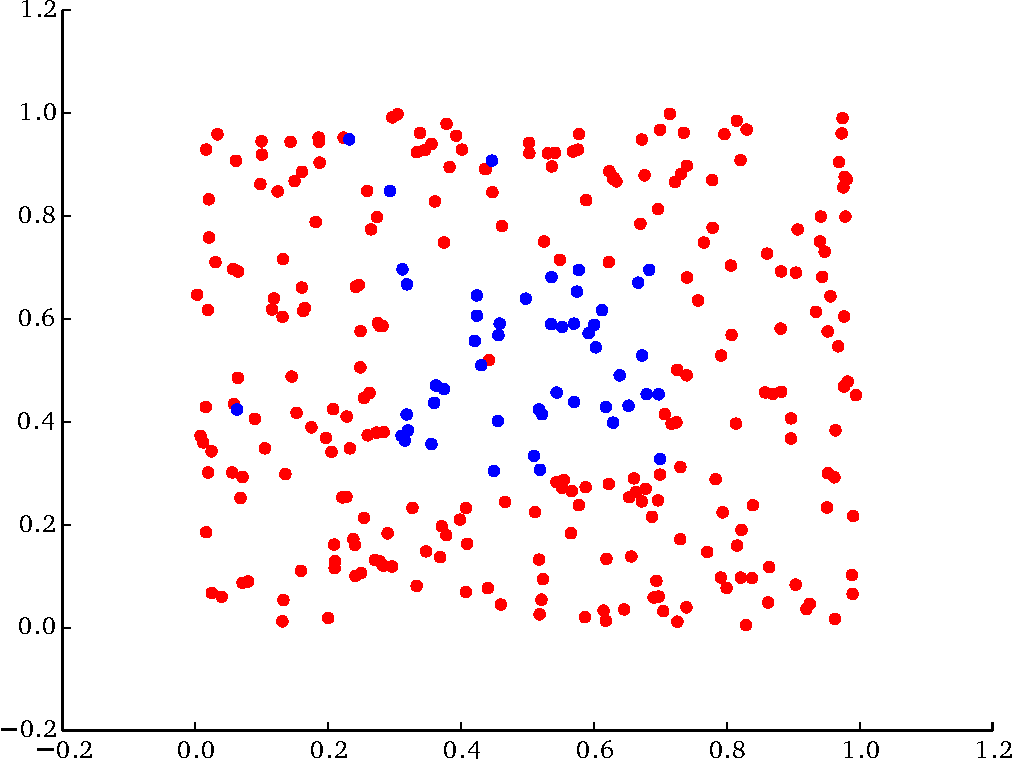
\includegraphics[width=\textwidth]{figures/ch5_learningset.pdf}
    \caption{Binary classification task.}
    \label{fig:5:set}
\end{minipage}\hfill
\begin{minipage}{0.45\textwidth}
\centering
    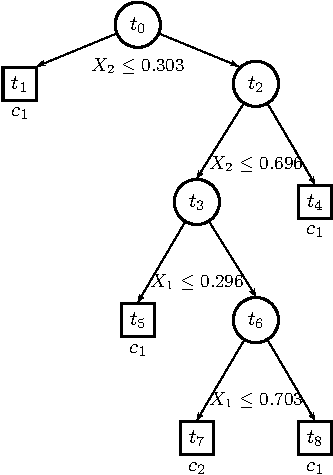
\includegraphics[scale=1.0]{figures/ch5_tree.pdf}
    \caption{Decision tree learned from Figure~\ref{fig:5:set}.}
    \label{fig:5:tree}
\end{minipage}
\end{figure}

As an example, Table~\ref{table:tree-array} illustrates the array
representation of the decision tree shown in Figure~\ref{fig:5:tree}, as built
from the learning set ${\cal L}$ of Figure~\ref{fig:5:set}. Internal nodes
($t_0$, $t_2$, $t_3$ and $t_6$) are nodes for which the corresponding values in
$\texttt{left\_child}$, $\texttt{right\_child}$, $\texttt{feature}$ and
$\texttt{threshold}$ are not empty, while leaves ($t_1$, $t_4$, $t_7$ and
$t_8$) correspond to nodes for which these values are not defined. In the case
of classification, the \texttt{value} array contains the number of samples of
each class for each node. From these, class probability estimates $p_{\cal
L}(Y=c|t)$ can be computed by dividing \texttt{value[t][c]} by the number of
samples $\texttt{n\_samples[t]}$ in $t$. In the case of regression,
\texttt{value[t]} would  contain the average output value for the samples in
$t$. Finally, let us note that storing node impurities in the \texttt{impurity}
array is not strictly necessary, since these values are only used during
construction. Yet, storing them can prove to be valuable, e.g., for
later inspection of the decision tree or for computing variable importances (see
Chapter~\ref{ch:importances}) more readily.

\begin{table}
    \small
    \hspace{-1.3cm}
    \begin{tabular}{| l | c c c c c c c c c |}
    \hline
    \texttt{t}    & 0 & 1 & 2 & 3 & 4 & 5 & 6 & 7 & 8 \\
    \hline
    \hline
    \texttt{left\_child} & 1 & -- & 3 & 5 & -- & -- & 7 & -- & -- \\
    \texttt{right\_child} & 2 & -- & 4 & 6 & -- & -- & 8 & -- & -- \\
    \texttt{feature} & 2 & -- & 2 & 1 & -- & -- & 1 & -- & -- \\
    \texttt{threshold} & 0.303 & -- & 0.696 & 0.296 & -- & -- & 0.703 & -- & -- \\
    \texttt{impurity} & 0.273 & 0. & 0.368 & 0.482 &  0.065 &  0.051 & 0.48  & 0.042 &  0. \\
    \texttt{n\_samples} & 300 & 99  & 201 & 113  & 88  & 38  & 75  & 46  & 29\\
    \texttt{value} & 251/49 & 99/0 & 152/49 & 67/46 & 85/3 & 37/1 & 30/45 & 1/45 & 29/0 \\
    \hline
    \end{tabular}
    \caption{Array representation of the decision tree in Figure~\ref{fig:5:tree}.}
    \label{table:tree-array}
\end{table}

By implementing the array representation as dynamic tables~\citep{cormen:2001},
insertion of new nodes has an $O(1)$ amortized cost, while keeping memory
allocations at a minimum and thereby reducing the overhead that would otherwise
occur using per-node data structures. Maintaining the representation
contiguously in memory also brings the benefits of leveraging CPU caches,
which might greatly improve performance when fast predictions are critical.
Since nodes are accessed successively and repeatedly at test time,
storing them in nearby memory locations is indeed highly recommended.

\subsection{Builders}

The implementation of the induction procedure in Scikit-Learn revolves around
three nested components:

\begin{enumerate}
\item The first component is a \texttt{Builder} object whose role is to
    effectively build the tree array representation presented above,
    by recursively partitioning nodes using splits found by a \texttt{Splitter} object.

\item The second component is a \texttt{Splitter} object whose role is to find splits on internal nodes.

\item The third component is a \texttt{Criterion} object whose role is to evaluate
    the goodness of a split.
\end{enumerate}

The most direct \texttt{Builder} implementation is the depth-first greedy
induction procedure as originally outlined in Algorithm~\ref{algo:induction}. A
critical aspect of this algorithm is how to keep account of the  the input
samples $(\mathbf{x},y) \in {\cal L}_t$  that arrive at node $t$. A
straightforward solution is to store lists of indices of the input samples at
node $t$. As pointed out in \citep{criminisi:2013}, building many such lists is
however inefficient because of repeated memory allocations and deallocations. A
better solution is to have instead all indices stored in a single static array
and to use in-place reordering operations when partitioning $t$. More
specifically, let assume that  $\texttt{samples}$ is the list of all indices
and that  $\texttt{start}$ and $\texttt{end}$ are bounds such that
$\texttt{samples[start:end]}$ contains the sample indices at the current node
$t$. If $\texttt{t}$ is split on feature $\texttt{feature[t]}$ and threshold
$\texttt{threshold[t]}$, then ${\cal L}_t$ can be partitioned into ${\cal
L}_{t_L}$ and ${\cal L}_{t_R}$ by reorganizing $\texttt{samples[start:end]}$
into $\texttt{samples[start:pos]}$ and $\texttt{samples[pos:end]}$, such that
all samples in the first part are on the left side of the split while all
samples in the second part are on the right side of the split. The induction
procedure then proceeds by pushing the bounds $\texttt{start:pos}$ and
$\texttt{pos:end}$ on the stack $S$, as an efficient way to effectively
represent ${\cal L}_{t_L}$ and ${\cal L}_{t_R}$.

An alternative implementation of the $\texttt{Builder}$ interface consists in
replacing the stack $S$ in Algorithm~\ref{algo:induction} by a priority queue,
hence changing the order in which the nodes are split. In particular, if nodes
$t$ are prioritized by weighted potential impurity decrease $p(t) \Delta
i(s^*,t)$ (where $s^*$ is the best split on $t$), then the greedy induction
procedure switches from a depth-first construction of the tree to a \textit
{best-first} induction procedure. In this way, an additional stopping criterion
can be defined as the maximum number \texttt{max\_leaf\_nodes} of leaves in the
tree. If nodes are expanded in best-first order, then the resulting tree only
includes the most significant splits, thereby pre-pruning all (seemingly)
irrelevant branches without wasting computational resources.

Likewise,  the stack $S$ in Algorithm~\ref{algo:induction} can be replaced by a
deque data structure, in which case the induction procedure switches to a
\textit{breadth-first} construction of the tree. With some modifications,
breadth-first construction shows to be more efficient when it is expensive to
randomly access the data~\citep{criminisi:2013}, e.g., when data are too big to
fit into memory and must be streamed from disk. Breadth-first induction also
proves to be an efficient strategy when combined with parallelism, e.g., for
building a whole level of the decision tree simultaneously using multiple
cores~\citep{liao:2013}.

\subsection{Splitters}

In Scikit-Learn, \texttt{Splitter} objects implement search procedures for
finding splits on internal nodes. In the case of decision trees, they implement
algorithms~\ref{algo:findsplit} and \ref{algo:findsplit:x_j} for finding the
best split over all $p$ input variables. In the case of randomized trees, they
implement the search procedure \ref{algo:findsplit:random} over $K \leq p$
randomly drawn input variables, combined with either algorithm
\ref{algo:findsplit:x_j} or  \ref{algo:findsplit:et} to respectively obtain
Random Forests or Extremely Randomized Trees. Again, several aspects of the
algorithm should be considered with care to obtain an efficient implementation:

\begin{description}

\item \textit{Data access.}\hfill\\
    Looking for the best split on the input variable $X_j$ and partitioning
    ${\cal L}_t$ requires to repeatedly access  over the node sample
    values $x_{i,j}$ (i.e., over values in the $j$-th column if samples are represented
    as a two dimensional array), which may comes at a non negligible cost if data is
    not ordered properly.  However, due to CPU caching and pre-fetching effects, the
    closer the values in memory, usually the lower it takes to access them. In
    our case, this can be exploited in two ways to minimize the cost of data access:

    \begin{itemize}
    \item By storing the learning set ${\cal L}$ using column-major order (i.e., Fortran
          array memory layout), hence storing the values $x_{i,j}$ of $X_j$ (for all samples $i=1,\dots,N$)
          contiguously in memory.
    \item By pre-fetching the node sample values $x_{i,j}$ (for $i = 1, \dots, N_t$) manually
          into a static and contiguous buffer, on which the search procedure
          is then applied.
    \end{itemize}

\item \textit{Sort algorithm.}\hfill\\
    In CART and Random Forests, finding the best split on $X_j$ requires
    to sort the sample indices $\texttt{samples[start:end]}$ along
    their respective values on $X_j$, i.e., such that
    \begin{align}
    \texttt{X[samples[start], j]} &\leq \dots \leq \texttt{X[samples[start+i], j]} \nonumber \\
                                  &\leq \dots \leq \texttt{X[samples[end-1], j]}, \nonumber
    \end{align}
    for $i=0,\dots,N_t-1$.
    As shown in Section~\ref{sec:5:complexity-fit},
    this operation drives the complexity of the overall induction procedure
    and  is therefore critical in the implementation of the algorithm.

    To guarantee the lowest time complexity in all cases, we rely on
    Introsort~\citep{musser:1997} which combines Quicksort and Heapsort into a
    hybrid sorting algorithm. Basically, sorting in Introsort begins with
    Quicksort and then switches to Heapsort when the depth of partitioning
    exceeds $\Theta(\log N)$. As such, the practical $\Theta(N\log N)$
    performance of Introsort is comparable to the average performance of
    Quicksort, except that performance in the worst case is bounded to
    $\Theta(N \log N)$  due to Heapsort, instead of $\Theta(N^2)$ in the
    worst case for Quicksort. Additionally, Quicksort is
    implemented using the median-of-three as pivot~\citep{bentley:1993}, hence
    yielding better partitions and further improving performance.

    \begin{figure}
        \centering
        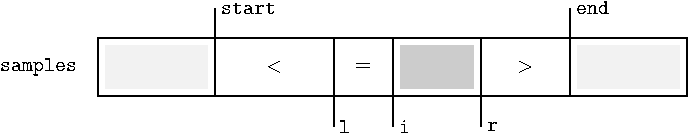
\includegraphics[width=0.9\textwidth]{figures/ch5_sort.pdf}
        \caption{3-way partition in Quicksort. Once $\texttt{i=r}$, elements that are identical
                 to the pivot are all set at their final positions \texttt{samples[l:r]}, in a single
                 recursive call. The sub-arrays \texttt{samples[start:l]} and \texttt{samples[r:end]}
                 are then recursively sorted.}
        \label{fig:5:sort}
    \end{figure}

    In the context of the tree induction procedure, let us finally notice that
    partitioning node samples ${\cal L}_t$ into subsets ${\cal L}_{t_L}$ and
    ${\cal L}_{t_R}$ not only makes them purer in terms of the ouput variable
    $Y$, it also indirectly makes node samples more and more identical in terms
    of the values taken by the input variables. As we get deeper into the tree,
    this property can be leveraged by implementing Quicksort as a 3-way
    recursive partition~\citep{bentley:1993}, as illustrated in
    Figure~\ref{fig:5:sort}. In this variant, elements that are identical to
    the pivot are all set at their final positions in a single recursive call,
    hence accelerating the sorting procedure. If the number of distinct values
    is constant, 3-way Quicksort can be shown~\citep{sedgewick:2011}
    to reduce running times from $O(N \log N)$ to $O(N H)$, where $H$ is the
    Shannon entropy defined on the frequencies of the values to be sorted. As a
    consequence, in the case of many duplicates (i.e., when $H=O(1)$),
    $c(N)=O(N)$ and using 3-way Quicksort for sorting the sample indices in
    fact reduces the overall complexity of Random Forests to the asymptotic
    complexity of Extremely Randomized Trees (see Section~\ref{sec:5:complexity-fit}).

\item \textit{Skipping locally constant input variables.}\hfill \\
    In the extreme case, recursively partitioning node samples might result in
    input variables $X_j$ to become locally constant at $t$. That is,
    $x_j=x^\prime_j$ for all $(\mathbf{x},y), (\mathbf{x}^\prime, y) \in {\cal
    L}_t$. In such  a case, there is no valid split on $X_j$ and trying to find
    one at $t$, but also at any of the descendant nodes, is a waste of
    computational resources. Accordingly, Algorithm~\ref{algo:findsplit:random}
    can be extended to account for variables that are known to be constant, thereby skipping
    non-informative variables if we know in advance that no valid split can be found.
    To stay as close as possible to the original algorithm, note however that constant
    variables are still included when drawing $K$ variables at random.

\item \textit{Split approximations.}\hfill\\
    In Chapter~\ref{ch:forest}, we showed that an increase of bias due to
    randomization is beneficial as long as it sufficiently decorrelates the
    predictions of the individual trees. Given this result, a legitimate
    question is to wonder if finding the very best splits $s^*_j$ really is
    imperative in the first place to achieve good accuracy in random forests. As proved by the
    good results usually obtained by Extremely Randomized Trees, even splits
    that are drawn at random are in fact often sufficient to reach good
    (sometimes even better) performance. More importantly, not only this yields
    comparable accuracy, it is also more computationally efficient. At midway
    between  exact best splits (as in Algorithm~\ref{algo:findsplit:x_j}) and
    random splits (as in Algorithm~\ref{algo:findsplit:et}), an intermediate
    and pragmatic solution is therefore to consider approximations of the best splits.
    The two most strategies are based on \textit{subsampling} and \textit{binning}:

    \begin{itemize}
    \item Let $N_0$ denote an upper limit on the node sample size. If $N_t > N_0$,
          the subsampling approximation of the best split $s^*_j$ at $t$ on $X_j$ consists
          in looking for the best split using only $N_0$ randomly drawn node
          samples from ${\cal L}_t$, and all node samples otherwise. The rationale behind this strategy is
          that, in the first nodes of the tree, the best splits are often
          so markedly superior to all other splits that this clear-cut information
          also reflects in a subsample. For nodes further down in the tree (i.e., for $N_t \leq N_0$),
          splits are usually less marked but then all node samples in ${\cal L}_t$
          are used, hence guaranteeing to find the same splits as in the original procedure.
          Historically, the subsampling strategy was first proposed in \citep{breiman:1984}
          in the context of single decision trees, for datasets too large to be held in memory.

    \item An alternative but close strategy is to consider only a subset
          of the possible discretization thresholds $v^\prime_k$ instead
          of exhaustively evaluating all candidate splits. In binning, this
          is performed by grouping together node samples that are close
          to each other into bins and then evaluating only the thresholds inbetween these groups.
          The simplest strategy of all is to divide the value interval of $X_j$
          at $t$ into $D$ intervals of equal length. Another strategy
          is to sort the node samples along their respective values of $X_j$
          and to partition them into $D$ subsets of equal size.
          More elaborate algorithms, also known as \textit{attribute discretization} procedures,
          are reviewed in \citep{zighed:2000}.
    \end{itemize}

\item \textit{Pre-sorting data.}\hfill\\
    As shown earlier, sorting node samples for each candidate split significantly impacts
    the overall complexity of the induction procedure. An alternative strategy is
    possible~\citep{breiman:2002} and consists in presorting the samples for all
    $p$ input variables before the construction of the tree. More specifically, let
    $i=1,\dots,\widetilde{N}$ denote the original indices of the unique input
    samples in ${\cal L}^m$. For each input variable $X_j$ (for $j=1,\dots,p$), the
    sorted indices $\sigma^j_1,\dots,\sigma^j_{\widetilde{N}}$, such that
    \begin{equation} x_{\sigma^j_1,j} \leq \dots \leq
    x_{\sigma^j_{\widetilde{N}},j}, \end{equation} can be computed in
    $O(p\widetilde{N}\log \widetilde{N})$. Given these indices, finding the best
    split at a node then simply amounts to iterate, in that order, over the
    samples $\smash{\sigma^j_1,\dots,\sigma^j_{\widetilde{N}}}$ (for all $K$ of the
    split variables $X_j$), which reduces complexity to
    $O(K\widetilde{N})$ instead of $O(K\widetilde{N}\log \widetilde{N})$.
    Partitioning the node samples into $t_L$ and $t_R$ then requires to partition
    all $p$ lists of sorted indices into $2p$ sub-lists of $\widetilde{N}_{t_L}$ and
    $\widetilde{N}_{t_R}$ sorted indices
    $\smash{\sigma^j_1,\dots,\sigma^j_{\widetilde{N}_{t_L}}}$ and
    $\smash{\sigma^j_1,\dots,\sigma^j_{\widetilde{N}_{t_R}}}$, which can be done in
    $O(p\widetilde{N})$. In total, the within-node complexity is
    \begin{equation}
    c(\widetilde{N}) = O(K\widetilde{N} + p\widetilde{N}) = O(p\widetilde{N}).
    \end{equation} Using this
    alternative strategy, the time complexity of RF for the best, the worst and the
    average cases is respectively $O(Mp\widetilde{N}\log \widetilde{N})$,
    $O(Mp\widetilde{N}^2)$ and $O(Mp\widetilde{N}\log \widetilde{N})$, as derived
    from theorems~\ref{thm:6:best:kn}, \ref{thm:6:worst:kn} and
    \ref{thm:6:average:kn} for $K=p$. Neglecting constant factors, the ratio between the two
    implementations is $O(\frac{p}{K\log \widetilde{N}})$, which might not necessarily
    lead to faster building times depending on $K$ and the size of the problem.

\end{description}

\subsection{Criteria}

The last components of the implementation of decision trees in Scikit-Learn are
\texttt{Criterion} objects for evaluating the goodness of splits. Supported
criteria are \texttt{"gini"} and \texttt{"entropy"} in classification, and the
reduction of variance \texttt{"mse"} in regression. All of them implement the
update mechanisms described in Section~\ref{sec:best-split-ordered}, such that
the iterative evaluation of $N_t-1$ splits on an ordered variable remains a
$O(N_t)$ operation.

\subsection{Parallelization}

Scikit-Learn implementation of random forests supports parallelism to
distribute computations on multi-core architectures. The simple, yet effective,
approach that we implement is to consider the construction of a forest as an
embarrassingly parallel problem, in which the $M$ decision trees are built
concurrently and independently on multiple processors. Assuming no overhead due
to parallelization, the theoretical speedup of this strategy is equal to the
number $N_p$ of processors used for building the forest. In practice however,
this upper bound is not always strictly reached due to the variance of the time
required for building randomized trees. It may indeed happen that building
trees take longer  than building some others, thereby underutilizing
computational resources since jobs may have finished sooner than others.

More fine-grained approaches consist in building decision trees one at time,
but using multiple processors. In the \textit{node-based decomposition}, the
construction of a tree is distributed by building multiple nodes concurrently.
In this case, workload can be divided between processors using a breadth-first
induction procedure and assigning whole sub-trees to develop once the waiting
queue contains $N_p$ nodes. Once again however, sub-trees may take longer to
build than others, hence underutilizing computational resources if the
resulting decision tree is not balanced. To alleviate this issue, processors
may be assigned single nodes to develop using a producer-consumer scheme to
balance workload in a fair way. Unfortunately, this latter approach often proves to be
dominated in practice by the overhead due to task assignment and bookkeeping
activities. Alternatively, the construction of a tree can also be distributed
using an \textit{attribute-based decomposition}. In this case, the workload is
divided by parallelizing the search of the $K$ best splits at a given node (see
Algorithm~\ref{algo:findsplit:random}). For detailed reviews on the topic, see
\citep{kufrin:1997,srivastava:2002}.

Using similar or hybrid approaches, let us finally note that the parallel
induction of random forests extend to other distributed architectures,
including GPUs~\citep{sharp:2008,liao:2013}, FPGA \citep{narayanan:2007} or
clusters \citep{mitchell:2011}.

% \begin{remark}{Multi-threading in Python}
% %\citep{masini:2011}
% \end{remark}


\section{Benchmarks}
\label{sec:5:benchmarks}

\subsection{Empirical complexity}

% Define some artifical data generators => regression + classification
% Regression: Friedman 1-2-3
% Classification: hastie_10_2, ringnorm, twonorm, threenorm, waveform
% http://www.cs.toronto.edu/~delve/data/datasets.html

% Evaluate the effect of
%   - M
%   - K
%   - bootstrap
%   - N
%   - p

%   - Unique values versus dupplicates
%   - sorting algorithm

% In classification, complexity should be proportional to the actual
% complexity of the capacity of the model to learn decision surface

% Measure
%   - Fit time
%   - Predict time
%   - Accuracy
%   - number of nodes
%   - average depth of nodes


\subsection{Comparison with other implementations}

Due to their relative simplicity, random forests have been reimplemented at
multiple occasions in various machine learning libraries and programming
languages. In this section, we compare the Scikit-Learn implementation
developed within this work with popular alternatives available in other machine
learning libraries and packages.

Table~\ref{table:implementations} summarizes the main open source
implementations of random forests along with some of their supported features.
All of them implement the original Random Forest algorithm~\citep{breiman:2001}
and therefore also provide an interface for Bagging~\citep{breiman:1996b} since
it corresponds to the special case $K=p$. Scikit-Learn, OpenCV and OK3 also
offer variants like Extremely Randomized Trees~\citep{geurts:2006} or Random
Subspaces\citep{ho:1998}. All support both classification and regression tasks,
with the exceptions of Weka and H2O which appear to only support
classification.

% by no means, this is an exhaustive list => there are domain specific impl (eg. random jungles) or proprietary impl (stalford, etc)

\begin{table}
    \footnotesize
    \centering
    \rotatebox{90}{
    \begin{tabular}{| c | m{1.5cm} >{\centering}m{0.8cm} m{1.4cm} m{2.5cm} >{\centering}m{1.8cm} >{\centering}m{0.8cm} >{\centering}m{0.8cm} >{\centering}m{1.3cm} m{3.5cm} |}
    \hline
        \textbf{Library} & \textbf{Algorithms} & \textbf{Tasks} & \textbf{Impurity} & \textbf{Stopping criteria} & \textbf{Variable importances} & \textbf{Multi-thread} & \textbf{Open source} & \textbf{Language} & \textbf{Reference} \\
    \hline
    \hline
    \textit{Scikit-Learn} & Bagging, RF, ETs, RS, RP & C/R & Gini, Entropy, MSE & \texttt{max\_depth}, \texttt{min\_samples\_split}, \texttt{min\_samples\_leaf}, \texttt{max\_leaf\_nodes} & \cmark & \cmark & BSD & Python & \citep{pedregosa:2011} \\
    \textit{randomForest} & Bagging, RF & C/R & Gini & \texttt{nodesize}, \texttt{maxnodes} & \cmark & \xmark & GPL & R & \citep{liaw:2002} \\
    \textit{Weka} & Bagging, RF & C & Gini & \texttt{depth}  & \xmark & \cmark & GPL & Java & \citep{hall:2009} \\
    \textit{OpenCV} & Bagging, RF, ETs & C/R & Gini & \texttt{max\_depth}, \texttt{min\_samples\_count}, \texttt{forest\_accuracy} & \cmark & \xmark & BSD & C/C++ & \citep{bradski:2008} \\
    \textit{OK3} & Bagging, RF, ETs & C/R & MSE & \texttt{varmin},\newline \texttt{nmin} & \cmark & \xmark & Source-available & C & \citep{geurts:2006} \\
    \textit{H2O} & Bagging, RF & C & Gini,\newline Entropy & \texttt{maxDepth}  & \xmark & \cmark & Apache & Java & \citep{vitek:2013} \\
    \textit{TMVA} & Bagging, RF  &  C/R & 0-1 loss,\newline Gini, Entropy, MSE & \texttt{NodePurityLimit}, \texttt{NNodesMax}, \texttt{MaxDepth} & \cmark & \xmark & BSD & C++ & \citep{hoecker:2007} \\
    \textit{Orange} & Bagging, RF & C/R & GainRatio, Gini,\newline Relief, MSE & \texttt{worst\_acceptable}, \texttt{min\_susbet}, \texttt{min\_instances}, \texttt{max\_depth}, \texttt{max\_majority} & \xmark & \xmark & GPL & Python & \citep{demsar:2013} \\
    \hline
    \end{tabular}}
    \caption{Popular libraries for random forests.}
    \label{table:implementations}
\end{table}

% Compare
%   - Scikit-Learn                OK
%   - Weka                        OK  => à corriger pour retirer le biais
%   - randomForest (R)            OK  => à corriger
%   - OpenCV                      OK  => à corriger
%   - Pierre                      OK
%   - H20                         None
%   - TMVA                        https://dbaumgartel.wordpress.com/2014/03/14/machine-learning-examples-scikit-learn-versus-tmva-cern-root/
%   - Orange?                     http://orange.biolab.si/doc//reference/matrix.htm

% Make a table of supported features
% Comparison on various datasets (time, accuracy)
% Discussion of the results

